% \documentclass{article}
% \usepackage{amsmath} % Pakiet do wyrażeń matematycznych
% \usepackage{graphicx} % Pakiet do grafiki

% \begin{document}

% \title{Zadanie}
% \author{Justyna Michalik}
% \date{1 listopad 2024}
% \maketitle

\section{Justyna Michalik}

\subsection{Wyrażenie matematyczne}
\begin{equation}
    E = mc^2
\end{equation}
Jest to słynne równanie Einsteina łączące masę i energię.

\subsection{Obraz}

\begin{figure}[H]
    \centering
    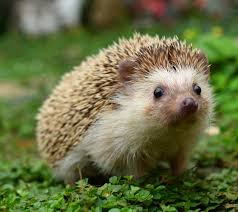
\includegraphics[width=0.5\textwidth]{pictures/pobrane.jpg}
    \caption{jeż}
    \label{fig:jeż}
\end{figure}

\subsection{fajne zwierzaki}
\subsubsection{Lista numerowana}
\begin{enumerate}
    \item jeż
    \item mrówka
    \item kotek
\end{enumerate}

\subsubsection{Lista nienumerowana}
ciastka zrobisz z:
\begin{itemize}
    \item mąka
    \item masło
    \item cukier
    \item mleko
    \item czekolada
\end{itemize}

\subsection{Tablica}
\begin{table}[H]
    \centering
    \begin{tabular}{|c|c|c|}
        \hline
        Kolumna 1 & Kolumna 2 & Kolumna 3 \\
        \hline
        1 & 2 & 3 \\
        4 & 5 & 6 \\
        7 & 8 & 9 \\
        \hline
    \end{tabular}
    \label{tab:przykladowa}
    
\end{table}


\subsection{Tekst}
Poniżej znajduje się przykładowy tekst z podstawowym formatowaniem. Jak widać, mamy tutaj dwa akapity z odwołaniem do rysunku \ref{fig:jeż} i tabeli \ref{tab:przykladowa}.

Pierwszy akapit wyjaśnia, że dokument zawiera różne elementy, takie jak wyrażenia matematyczne, obrazy, tabele oraz listy numerowane i nienumerowane. Każdy z tych elementów jest sformatowany zgodnie z zasadami LaTeX, co zapewnia spójny wygląd dokumentu.

Drugi akapit odnosi się do figury \ref{fig:jeż} i tabeli \ref{tab:przykladowa}, aby pokazać, jak w LaTeX odwoływać się do wcześniej wprowadzonych obiektów. To ułatwia organizację i nawigację po treści.

% \end{document}

